% !TeX root = ../main.tex
\documentclass[
    ngerman,
    accentcolor=3b,
    dark_mode,
    fontsize= 12pt,
    a4paper,
    aspectratio=169,
    colorback=true,
    fancy_row_colors,
    leqno,
    fleqn,
    boxarc=3pt,
    fleqn,
    % shell_escape = false, % Kompatibilität mit sharelatex
]{algoslides}

%%--------------------------%%
%%--Imports from Main File--%%
%%--------------------------%%
\usepackage{import}
% Import all Packages from Main Preamble with relative Path (buggy, list packages instead)
\subimport*{../shared}{preamble}
% Get Labels from Main Document using the xr-hyper Package
\externaldocument[ext:]{../main}
% Set Graphics Path, so pictures load correctly
\graphicspath{{../pictures}}
\def\codeDir{../code}

\begin{document}
    \section{Vor- und Nachteile von \LaTeX}\label{2}\label{2}
    \subsection{Vorteile}\label{2.1}\label{2.1}
    \begin{frame}
        \slidehead{}
        \begin{itemize}
            \item Einfache (nachträgliche) Änderung des Design
            \item Automatisierung
                \begin{itemize}
                    \item Seitennummer,
                    \item Inhaltsverzeichnis,
                    \item Abbildungsverzeichnis,
                    \item Literaturverzeichnis,
                \end{itemize}
            \item Fußnoten, Referenzen, Formatierung, $\dots$ sind einfach zu managen
            \item Formeln zu tippen ist intuitiv und einfach
            \item Stabil auch bei sehr großen Dokumenten
            \item Plattformunabhängig\begin{itemize}
                    \item Linux: TeXLive
                    \item Windows: TexLive oder MikTex
                    \item MacOS: TeXLive
                \end{itemize}
            \item Viele nützliche Pakete, die einem das Leben einfach machen
        \end{itemize}
    \end{frame}
    \begin{frame}[c]
        \begin{figure}[ht!]
            \centering
            \colorbox{white}{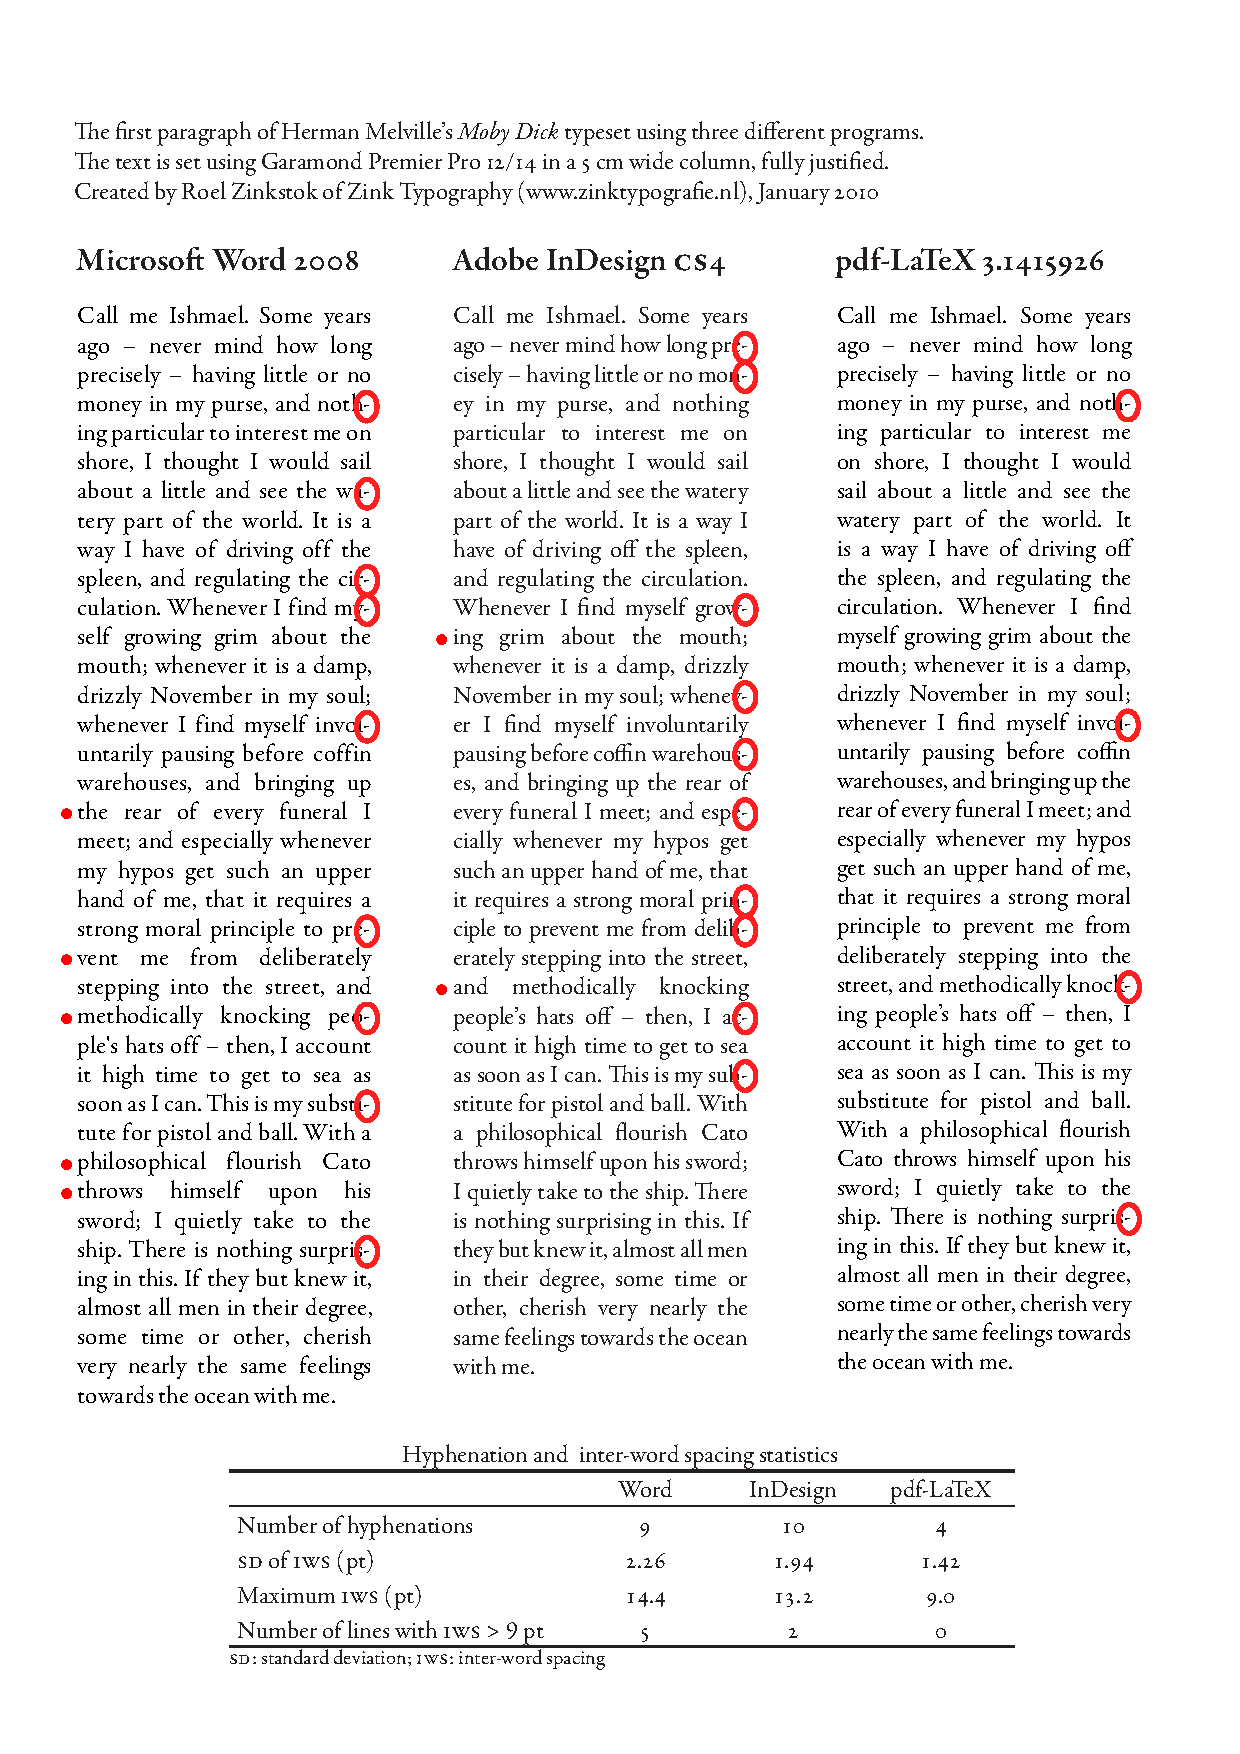
\includegraphics[height=6.5cm]{LaTeX vs Word vs Indesign.pdf}}
            \caption{Vergleich von \LaTeX, Word und InDesign}
            \label{fig:LaTeX-Vergleich}
        \end{figure}
    \end{frame}
    \subsection{Nachteile}\label{2.2}\label{2.2}
    \begin{frame}
        \slidehead{}
        \begin{itemize}
            \item Ungewohnt (auch wenn man schon einige Programmier- und Markup Sprachen kennt)
            \item Kein WYSIWYG (What you see is what you get)
                \begin{itemize}
                    \item Bis man Änderungen sieht kann lange dauern (gerade bei großen Dokumenten)
                \end{itemize}
            \item Steile Lernkurve
            \item Mehr Text, um Dinge zu beschreiben
        \end{itemize}
    \end{frame}
    \subsection{Komplexität}\label{2.3}\label{2.3}
    \begin{frame}
        \slidehead{}
        \tikzset{
            mylegend/.style={
                fgcolor,
                fill=\IfDarkModeTF{.!20!\thepagecolor}{.!20!\thepagecolor},
                fill opacity=0.9,
                draw=none,
                draw opacity=1,
                text opacity=1,
                rounded corners=3pt,
            },
        }
        \begin{figure}[ht!]
            \centering
            \begin{tikzpicture}
                \begin{axis}[
                        axis lines=center,
                        width=12cm,height=6cm,
                        xmin=0,
                        xmax=10,
                        ymin=0,
                        ymax=4,
                        xlabel={Komplexität des Dokuments},
                        ylabel={Aufwand},
                        legend style={
                            mylegend,
                            % at={(0.18,0.71)},
                            % anchor=north west
                        },
                        ticks=none,
                    ]
                    \addplot[samples=100,smooth, TUDa-3a,thick] coordinates {
                        (0,0.4)
                        (.5,2)
                        (2,2.3)
                        (5,2.5)
                        (10,2.8)
                    };
                    \addlegendentry{\LaTeX};
                    \addplot[samples=100,smooth, TUDa-8a,thick] coordinates {
                        (0,0.2)
                        (2,.5)
                        (4,2.5)
                        (8,8.6)
                    };
                    \addlegendentry{Word};
                \end{axis}
            \end{tikzpicture}
            \caption{Dokumentenkomplexität \LaTeX vs Word}%
            \label{fig:latex_vs_word}
        \end{figure}
    \end{frame}
\end{document}
